\newcount\Comments  
\Comments=1   
\documentclass[a4paper,12pt, english]{article}
\usepackage[top=2cm, bottom=2cm, left=2cm, right=2cm]{geometry}

\usepackage{babel}
%\usepackage{amsmath}
\usepackage{listings}

\usepackage{color}

\definecolor{darkgreen}{rgb}{0,0.5,0}
\definecolor{purple}{rgb}{1,0,1}
%\usepackage{subcaption}

\newcommand{\kibitz}[2]{\ifnum\Comments=1\textcolor{#1}{#2}\fi}
% add yourself here:
\newcommand{\ls}[1]{\kibitz{red}      {[Larisa: #1]}}
\newcommand{\cg}[1]  {\kibitz{purple}   {[Crina: #1]}}
\newcommand{\ns}[1]{\kibitz{cyan}     {[Noureddin: #1]}}


\usepackage{graphicx}
\usepackage{caption}

\usepackage{listings}
\usepackage{url}
%\usepackage{graphicx}

\usepackage{verbatim}

%\usepackage{caption}
%\usepackage{enumitem}

%\onehalfspacing

\begin{document}

\title{Regression Analysis}
%\date{Mar 2014}
%\author{By: Noureddin Sadawi}
\maketitle

\section{Introduction}
Regression analysis is a powerful technique that can be used to address various research questions. In this report, we are going to use it to check how q levels are affected by cu and phi. In particular, the type of regression we are going to use is "Multiple Linear Regression". Linear regression is the process of finding the best-fitting straight line through data points (this line is sometimes referred to as the regression line). Multiple means we have more than one input variable (also known as predictor), hence, we are trying to fit a plane or hyper-plane rather than a line.  The input variables in our case are cu, phi and as. Linear means that we are trying to find a combination of the input variables such that each variable is multiplied by a coefficient and then we sum the products. The idea is to use this linear combination of input variables to model their relationship with an output variable (in our case, this is q).

\section{The Modelling Tool}
In order to fit models, we are going to use R~\cite{R} which is a powerful and easy to use tool for statistical computing and graphics. R makes it easy to manipulate data and perform calculations as well as display information graphically. It also facilitates modelling (linear and nonlinear) and other statistical processes.
\section{Plotting the Data}
\begin{figure}[b]
  \centering
  
\includegraphics[width=0.5\textwidth]{pairs}
  \caption{A gull}
  \label{fig:pairs}
\end{figure}

\section{Examining a Fit}
There are several diagnostics that can be used to explore the goodness of fit of a model. In the remainder of this report we are going to use the following:
\subsection{R-squared}
This value calculates the percentage of variation of the output explained by the input variables in the model. This means the higher the value of R-squared the better the model. 
\subsection{R-squared adjusted}
This value is similar to R-squared but it accounts for the number of input variables in the model, hence, it is sometimes preferred to R-squared.
\subsection{Residuals}
A residual is the difference between the actual value and predicted value for each point (or record) in the data. Histograms are often used to check the distribution of residuals. Also, they are plotted against each input variable. If a model fits well, the residuals will be small and will be no pattern of their distrbution around zero (i.e. they should be evenly spread around zero).
\subsection{Deviance}
\subsection{Bayesian Information Criterion}

\section{Fitting the Models}
Let us begin fitting and examining the models. In the following subsections, we are going to fit all possible combinations of our three input variables.
\subsection{cu vs q} 
In this section, we are going to build a simple linear regression model using just cu as input and q as output. After using R's lm() function, the model looks as follows:\\
\begin{equation}
\label{eq:cu}
q = 92.890    +    8.557*cu 
\end{equation}       
By examining equation~\ref{eq:cu}, we observe that an increase, of decrease, of cu by one unit, causes an increase, or decrease, in q by 8.557 units
\begin{figure}[h!]
  \centering
  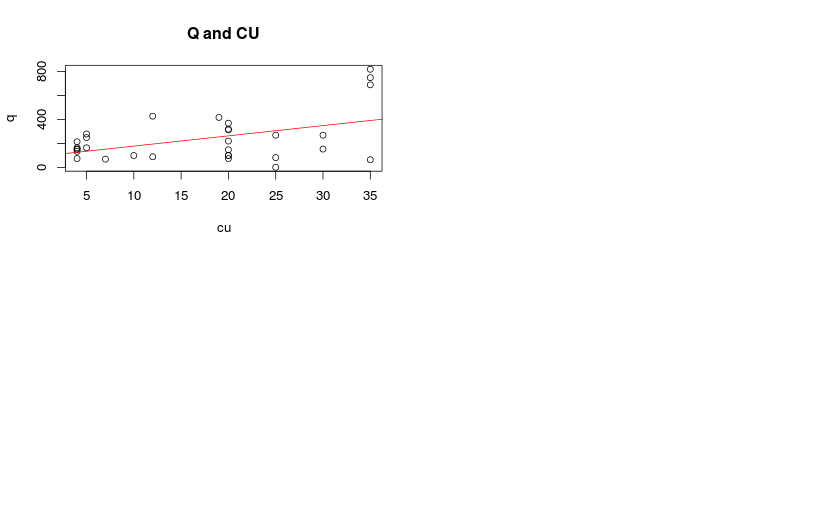
\includegraphics[width=0.6\textwidth]{cu-line}
  \caption{A gull}
  \label{fig:cu-line}
\end{figure}

Let us examine Figure~\ref{fig:cu-goodness}. The top-left plot shows a standard residual plot displaying residuals against fitted values. The labelled points are considered to be outliers. We do not observe any apparent pattern in the points on this plot. The top-right plot is a Q-Q plot of standardized residuals. As we can observe, the errors are approximately normally distributed. The bottom-left plot is a Scale-Location which is the same as standard residual plot (both show no trend to the residuals). The bottom-right plot shows residuals vs. leverage. Any labeled points on this plot should be investigated as they can possibly be having undue influence on the regression relationship.\\
Points 17,23,25 REMOVE?


\begin{figure}[h!]
  \centering
  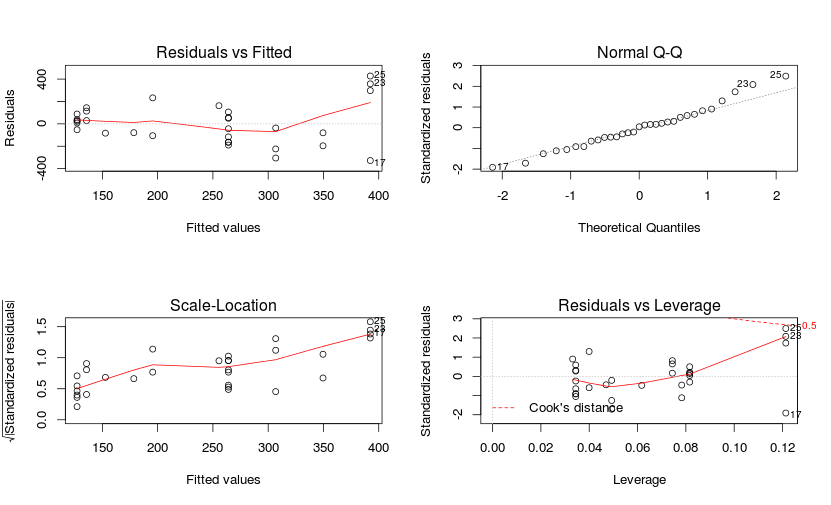
\includegraphics[width=0.6\textwidth]{cu-goodness}
  \caption{A gull}
  \label{fig:cu-goodness}
\end{figure}


\bibliographystyle{plain}
\bibliography{report}
\end{document}

